\documentclass[12pt]{article}

% taken from APL Memo style
\topmargin      -1in 
\marginparsep   0in
\headheight     .75in  
\headsep        0.25in
\textheight     9in 
\oddsidemargin  0in 
\evensidemargin 0in 
\textwidth      6.50in 

\pdfoptionpdfminorversion=6

\usepackage[hyphens]{url}
\usepackage{hyperref}
\usepackage{subcaption}
\usepackage{fancyhdr}
\usepackage[usenames,dvipsnames]{color}
\usepackage{listings}  
\usepackage{cite}
\usepackage{graphicx}
\usepackage{mathptmx}
\usepackage{acronym}
\usepackage{array}
\usepackage{gensymb}
\usepackage[toc,page]{appendix}
\usepackage{color, colortbl}
\usepackage{multirow}
\usepackage{booktabs}
\usepackage{gensymb}
\usepackage[nottoc]{tocbibind}
\usepackage{hyperref}
\usepackage{cleveref}
\usepackage{pifont}
\usepackage{array}

\definecolor{Gray}{gray}{0.9}

\newcommand\MyBox[2]{
	\fbox{\lower0.75cm
		\vbox to 1.7cm{\vfil
			\hbox to 1.7cm{\hfil\parbox{1.4cm}{#1\\#2}\hfil}
			\vfil}%
	}%
}

\newcolumntype{L}{>{\centering\arraybackslash}m{3cm}}
\hypersetup{colorlinks=true, 
	 	    linkcolor=black, 
		    urlcolor=black, 
		    citecolor=black,
		    filecolor=black}
		    
\urlstyle{rm}

% add any other paths here where images might reside (ideally a relative path)
\graphicspath{ {images/} }

% for two-column references
% from: http://tex.stackexchange.com/questions/20758/bibliography-in-two-columns-section-title-in-one
%\usepackage{multicol}
%\usepackage{etoolbox}
%\patchcmd{\thebibliography}{\section*{\refname}}
%    {\begin{multicols}{2}[\section*{\refname}]}{}{}
%\patchcmd{\endthebibliography}{\endlist}{\endlist\end{multicols}}{}{}
\setlength{\parindent}{0in}

\acrodef{nlp}[NLP]{Natural Language Processing}
\acrodef{cnn}[CNN]{Convolutional Neural Network}
\acrodef{rnn}[RNN]{Recurrent Neural Network}
\acrodef{api}[API]{Application Programming Interface}
\acrodef{bow}[BOW]{Bag of Words}
%%% paragraph spacing
%\setlength{\parindent}{4em}
\setlength{\parskip}{1em}

\begin{document}
\begin{titlepage}
	\centering
	
\includegraphics[width=\textwidth]{jhu_logo.png}\par\vspace{2cm}
	{\scshape\Huge Application of Convolutional Neural Networks to Natural Language Processing \\
	\vspace{1.5cm}
	 \scshape\Large EN.525.801(21) - Special Project I Summer 2016\par}
	{\scshape \Large Austin Dress\par} 
	\vspace{0.75cm}
%	{\scshape \Large DRAFT\par}
	\vfill
	{\large \today\par}
\end{titlepage}

\tableofcontents
\listoftables

\newpage

\section{Preface} 
\ac{nlp} is a field in computer science that focuses on processing human language. Human language can be referred to as a natural language as it has evolved overtime without strict syntax rules that one would find in programming languages. A simple example of \ac{nlp} would be processing a sentence and identifying the verb, subject, adjective. Writing a program to process a scholarly article and generate a summary would be a more advanced application.

In recent years \ac{cnn}s, a deep learning technique for image recognition, have gained huge popularity after Alex Krizhevsky won the Imagenet LSVRC2012 competition with his network \cite{alex}. Since then \ac{cnn}s have shown promising results in many other domains such as audio processing and \ac{nlp}. 

Over the course of the semester I explored using Word2Vec \cite{word2vec} to create word embeddings and then train a \ac{cnn} on the embeddings for sentiment analysis of various datasets. This document captures topics in \ac{nlp} that I explored throughout the semester, and my classification results for two datasets.

\section{Development Schedule}

In \cref{App:AppendixA} the development schedule is shown for the semester. This chart was created as a way to set short term goals for the semester to keep myself on task. The semester is broken down into research, testing and evaluation, and finally documentation and presentation at the end of the semester. 

\section {Background and Previous Work} \label{background}
Prior to beginning the semester I had very little experience with \ac{nlp} and thus needed to do some reading on how traditional classifiers are built for sentiment analysis. In this section I cover data preparation that is necessary in any \ac{nlp} task as well as two word embedding techniques. Word embeddings are number representations of words. When training a classifier for any type of task the input is usually a feature vector containing floating point numbers and integer labels. Word embeddings are needed as raw ascii characters are not valid inputs for classifiers.

\subsection {Data Pre-processing and Cleaning}
In any type of machine learning task data pre-processing is typically required. For example, in image processing the input image may be pre-processed by convolving a gaussian kernel and normalizing the image to remove noise. In \ac{nlp} similar types of pre-processing are required. Take for example the following Twitter tweets from the Sentiment140 dataset \cite{sentiment140}:

\begin{enumerate}
	\item \#poemsunder140 ....started by \@shannonelyse1
	\item Juuuuuuuuuuuuuuuuussssst Chillin!!
	\item :-D ))))))))...WHAT AN AMAZING NIGHT,DAY \&amp; NIGHT AGAIN!! HI TWITS! I MiSS U GUYS"
	\item @dandelionas is making fettucini and garlic bread!
\end{enumerate} 

Twitter tweets contain text fields known as ``hash tags", a phrase proceeded by a ``\#" symbol, and an ``at" symbol, a username proceeded by an ``@" symbol. Tweets 1 and 4 contain such information and for the purposes of sentiment analysis are extraneous as hastags and twitter usernames do not affect sentiment. In addition, repeated letters in words, capitalization, punctuation marks, and emoticons are removed. Prior to being passed to a classifier for training or testing these tweets would be converted to the following (as an example): 

\begin{enumerate}
	\item started by
	\item just chillin
	\item what an amazing night day night again hit twits i miss u guys
	\item is making fettucini and garlic bread
\end{enumerate} 

This cleaning and preprocessing step is typically exploits regular expressions to quickly locate the patterns previously mentioned and remove them. Spelling and grammer correction are typically not applied. 

\subsection{Co-occurence Matrices}

A co-occurence matrix is one method for representing a word as a vector. These matrices use the surrounding words in a sentence to represent a word. This matrix captures the number of times a other word occurs directly next to it in a dataset. For example in the Standford Deep Learning Course \cite{dl_course}, they show the following example:

\begin{itemize}
	\item I like deep learning.
	\item I like NLP.
	\item I enjoy flying.
\end{itemize}

\begin{figure}[htbp!]
	\centering
	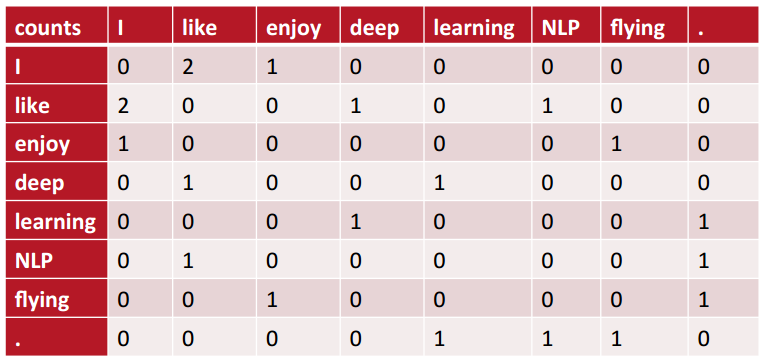
\includegraphics[scale=.4]{cooccurence.png}
	\caption{Co-occurence Matrix example.}
	\label{fig:cooccurence}
\end{figure}

This matrix shown in Figure \ref{fig:cooccurence} displays the number of times words appear next to each other in the three sentences above. The idea is that each row represents a feature vector that characterizes each word in the whole dataset.

There are obvious drawbacks to representing words in this way. One being that as the number of words in the dataset increases, so does the dimensionality of the matrix. Representing words in this way allows us to create a similarity metric between words as words in human language tend to appear next to each other. In Section \ref{word2vec} the Word2Vec word representation is covered. Word2Vec is a more state of the art word representation technique.

\subsection {Bag of Words}

The \ac{bow} algorithm is used in many \ac{nlp} applications such as sentiment analysis and also has applications in image processing. The general algorithm is described as it was used as a baseline for the two datasets used during the semester. The \ac{bow} algorithm and its word representation is  fairly intuitive. As an example take the common American English language tongue-twister and its response:

\begin{enumerate}
	\item How much wood could a woodchuck chuck if a woodchuck could chuck wood?
	\item A woodchuck would chuck as much wood as a wouldchuck could chuck if a woodchuck could chuck wood.
\end{enumerate} 

From these two sentences a vocabulary, or word corpus, can be built. For these two phrases the corpus would be: \{\textit{how, much, wood, could, a, woodchuck, chuck, if, would, as}\}.

\ac{bow} builds a feature vector for a sentence, paragraph, or document by counting the number of time a given word appears. For the two phrases listed above the feature vector representations would be as follows:

\begin{enumerate}
	\item \{1,1,2,2,2,2,2,1,0,0\}
	\item \{0,1,2,2,3,3,3,1,1,2\} 
\end{enumerate} 

One of the nice features of \ac{bow} is that the feature vectors produced by it are always the same length. The main downfall of the \ac{bow} is that as the corpus size increases so does the dimensionality of the feature vector. This results in feature vectors that are very sparse. For example, training \ac{bow} on the Twitter tweets would result in feature vectors with many zeros as tweets are limited to 140 characters. It is for this reason that a corpus size limit of, for example 5000 words is enforced. 

\section{Word2Vec} \label{word2vec}

Word2Vec \cite{word2vec} is an unsupervised learning technique for generating word embeddings developed in C++ by Google. Word2Vec is similar to co-occurence matrices previously mentioned, but produces very dense word vector representations. These word vectors contain rich information about how they relate to other words. This concept is similar to finding a strong correlation between neighboring pixels in an image. In the case of an image, RGB values are known already. In a sentence it is clear to a human that there is correlation between words, but capturing this information in a vector space is challenging. Word2Vec is one solution to this problem, though there are others, such as GloVe \cite{pennington2014glove} researched at Stanford.

Training a Word2Vec model is as simple as taking a text dataset, preprocessing it, and feeding the sentences into the training function. The Gensim \cite{rehurek_lrec} library was utilized to train and test Word2Vec models. Gensim is a Python wrapper around Google's C++ code that makes setting up data and training a model easier.

Prior to training a Word2Vec model Gensim requires that several parameters be set:

\begin{table}[!htbp]
	\centering
	\footnotesize
	\begin{tabular}{|>{\raggedright\arraybackslash}m{30mm}|m{70mm}|m{20mm}|m{20mm}|}
		\hline
		\rowcolor{Gray}
		\multicolumn{1}{|>{\centering\arraybackslash}m{30mm}|}{\textbf{Parameter}} 
		& \multicolumn{1}{>{\centering\arraybackslash}m{70mm}|}{\textbf{Description}} 
		& \multicolumn{1}{>{\centering\arraybackslash}m{20mm}|}{\textbf{Typical Value}}\\ \hline
		num\_features       & Word Vector Dimensionality & 300          \\ \hline
		min\_word\_count   &  Minimum number of times word must appear to be included & 40          \\ \hline
		context  & Context window Size     & 10     \\ \hline
		downsampling & Downsample setting for frequent words           & 1e-3           \\ \hline
	\end{tabular}
	\caption{Input parameters for training a Word2Vec model.}
	\label{table:gensim_inputs}
\end{table}

The values shown in Table \ref{table:gensim_inputs} are the main tunable parameters for the algorithm. In general 300 feature dimensions produces good results. The minimum word count is a good way to remove words that are misspelled. 

\begin{figure}[htbp!]
	\centering
	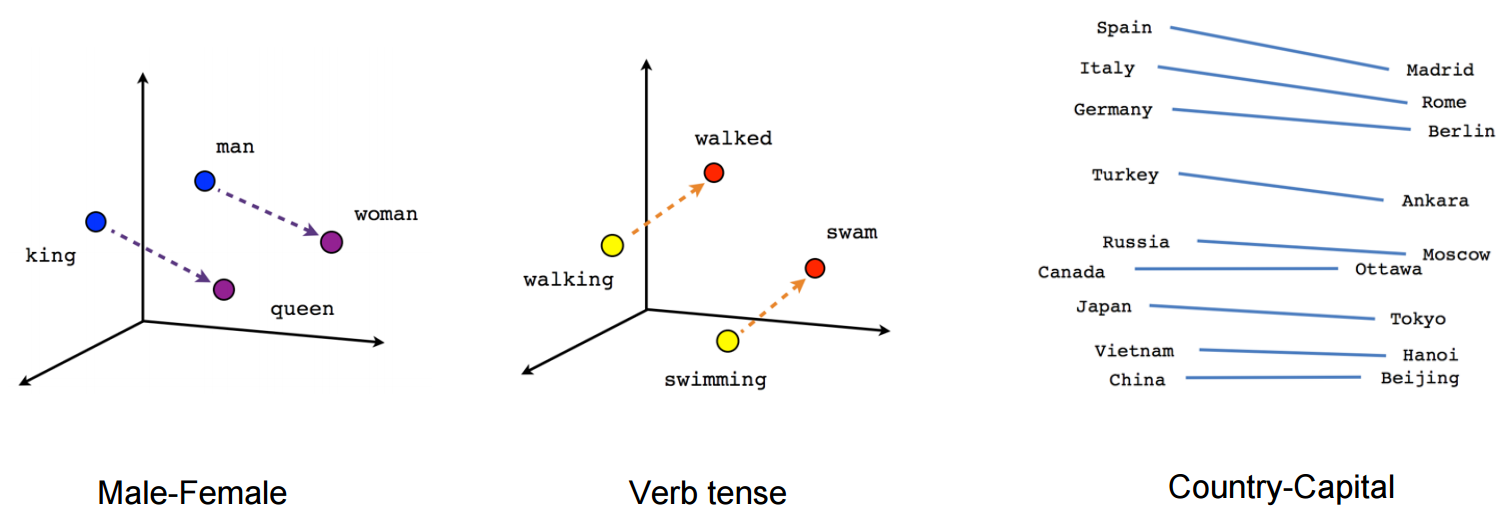
\includegraphics[scale=.3]{linear-relationships.png}
	\caption{Word vector visualization \cite{tensorflow} showing semantic relationships between words.}
	\label{fig:linear-relation}
\end{figure}

Figure \ref{fig:linear-relation} and Appendix \ref{App:AppendixB} show words plotted in feature space after dimension reduction and projection. These plots show the power of Word2Vec word embeddings as similar words are spatially close to each other. Performing vector addition and subtraction reveals interesting properties. Specifically the embeddings are able to capture analogies. Below are several screenshots showing some of the unique properties or word vectors. These results were generated by training a Word2Vec model on the Sentiment140 dataset.

\begin{figure}[htbp!]
	\centering
	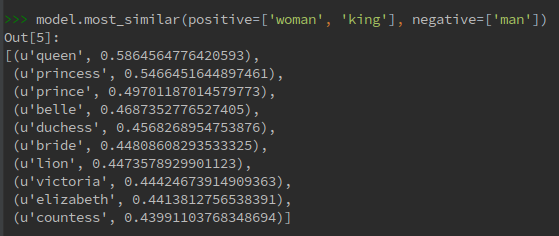
\includegraphics[scale=.5]{man_woman.png}
	\caption{Example of Word2Vec vector addition and subtraction.}
	\label{fig:man_woman}
\end{figure}

In Figure \ref{fig:man_woman} vector addition and subtraction of word vectors is shown: woman + king - man. The output of the model suggests the top 10 closest words in the vector space. Queen is the closest in the feature space and is likely the answer that human would give to this analogy.

\begin{figure}[htbp!]
	\centering
	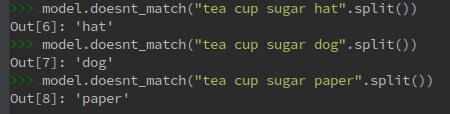
\includegraphics[scale=.5]{tea_cup.png}
	\caption{Word2Vec determining which word does not belong.}
	\label{fig:tea_cup}
\end{figure}

Related words are closely spaced in feature space which makes it possible to do other interesting tasks such as identifying words that do not belong in the same set/classification. Figure \ref{fig:tea_cup} shows that Word2Vec embeddings can correctly identify that the words \{hat, dog, paper\} do not belong to the same set of words \{tea, cup, sugar\}.


\section {Keras: Designing a CNN Network for Sentence Classification}
Keras \cite{chollet2015keras} is one of the many nerual network frameworks available for deep learning. Keras is modular, GPU accelerated, and supports \ac{cnn}s, \ac{rnn}s, and standard neural networks. At its core Keras, is a python wrapper around the Theano and TensorFlow deep learning frameworks. I decided to use this tool to construct \ac{cnn}s due to it's flexibility and rapid prototyping capability. Changing the number of filters in a \ac{cnn}, size, and\slash or number of fully connected layers is very simple. 

The general procedure for training a \ac{cnn} for text classification is as follows:

\begin{enumerate}
	\item Pre-process text dataset by cleaning as described in Section \ref{background}.
	\item Generate word embeddings for data using \ac{bow}, Word2Vec, raw number representations, or co-occurence matrices.
	\item Pass the entire training dataset through the network (epoch).
	\item After each epoch the calculate loss on training and validation datasets.
	\end{enumerate} 

\ac{cnn}s used for text classification are not very large when compared to those used for image processing. This is mainly due to the fact that in text classification there is only one channel and convolutions are 1-dimensional. The network architecture I used for both datasets is similar to networks used in early applications of \ac{cnn}s to text classification \cite{kim2014convolutional}. I used filter windows sizes of 3 and 4 words with 100 filters for each filter size. The outputs of the convolution process are feature maps which are then sent through a max-pooling layer. The outputs of the pooling layer are then sent to a fully-connected layer (standard neural network) with 100 neurons and softmax output. The output of the softmax layer is a probability for each class: positive or negative sentiment.

The structure in Figure \ref{fig:network_structure} is an example of a \ac{cnn} used for text classification. Each word in a sentence or document that is to be classified is converted into an embedded form using Word2Vec. The vector representations of each word generated by Word2Vec all have the same number of dimensions. A filter of size 3, for example, looks at 3 words at a time as it is convolved across a sentence or document. The output of each convolution step is a feature. When \ac{cnn}s are applied to images the input image must always be scaled to have the same width and height that the network expects. \ac{cnn}s used for text classification have the same requirement. The input size is calculated by counting the number of words in each exemplar in the dataset. The length of the longest document or sentence is then used as the input size. All sentences that are shorter than the longest exemplar are extended by using a padding word. A \ac{cnn} and Word2Vec will find no meaning in the padding word.

\begin{figure}[htbp!]
	\centering
	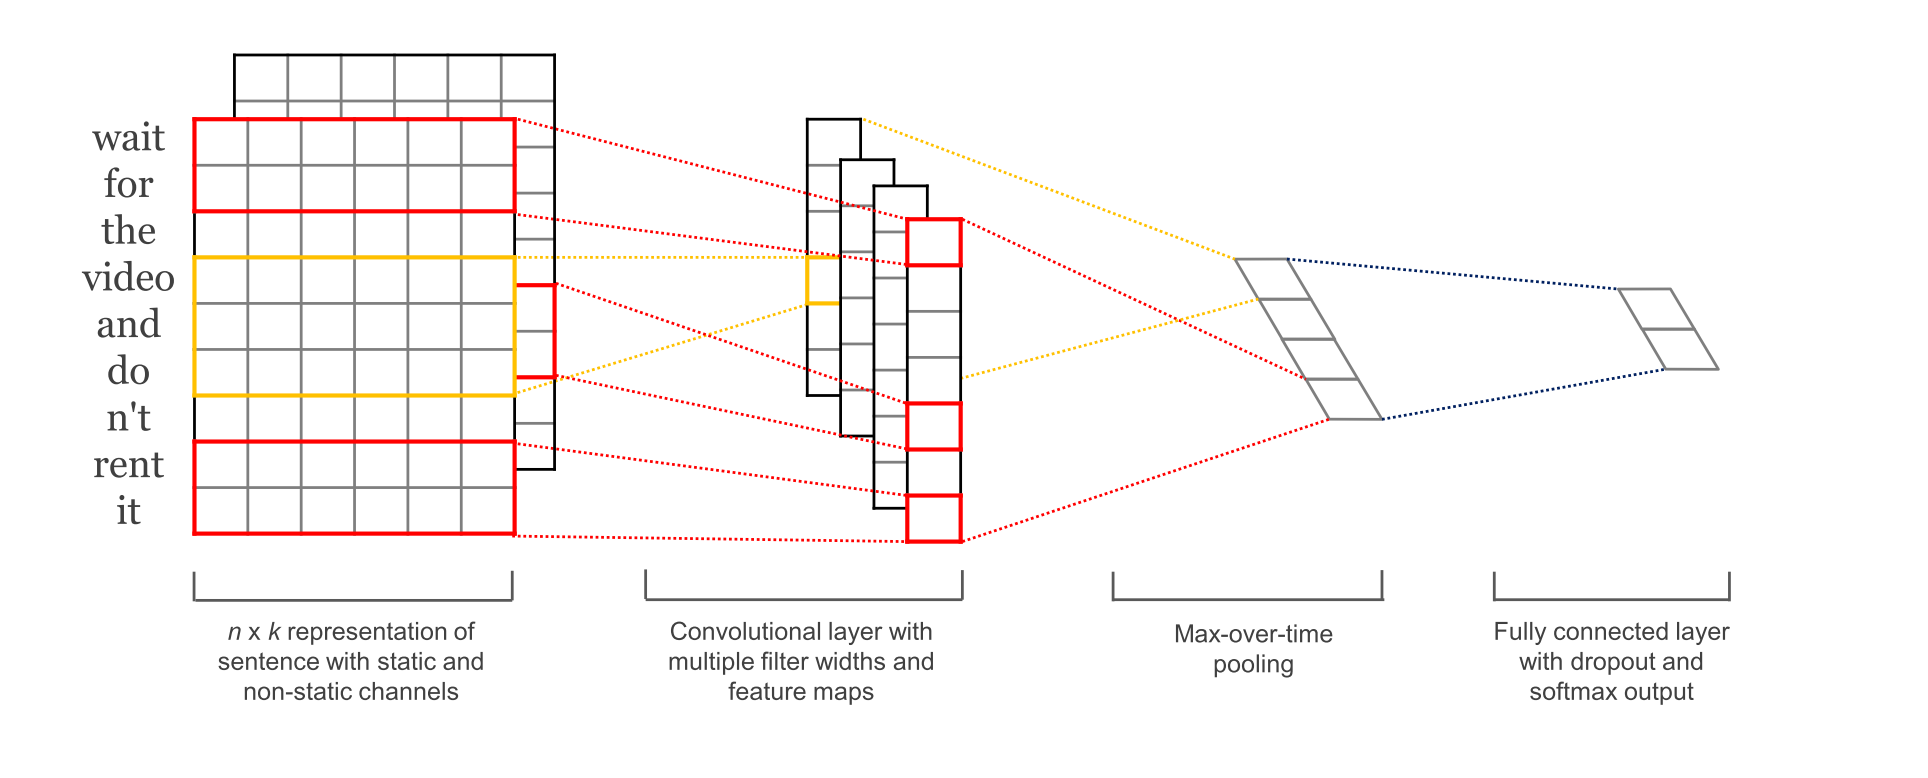
\includegraphics[scale=.4]{network_structure.png}
	\caption{Example \ac{cnn} architecture for sentence classification \cite{kim2014convolutional}.}
	\label{fig:network_structure}
\end{figure}

In Figure \ref{fig:training} the output of Keras during training is shown. In this case, the network was trained on a portion of the Twitter dataset for testing. At each epoch the entire dataset is pushed through the network. The loss and accuracy for both the training and validation sets are shown. In this example, the network's accuracy increases by about 1\% after each epoch. Each epoch takes about 41 seconds to complete on the GPU. No CPU mode timings were collected. The number of epochs is configurable. The networks trained for this research typically ran for only 7-10 epochs as validation set accuracy plateaued. Seeing the loss for validation and training sets is very important as it makes it clear if the model is overfitting to the training set.

\begin{figure}[!htbp]
	\centering
	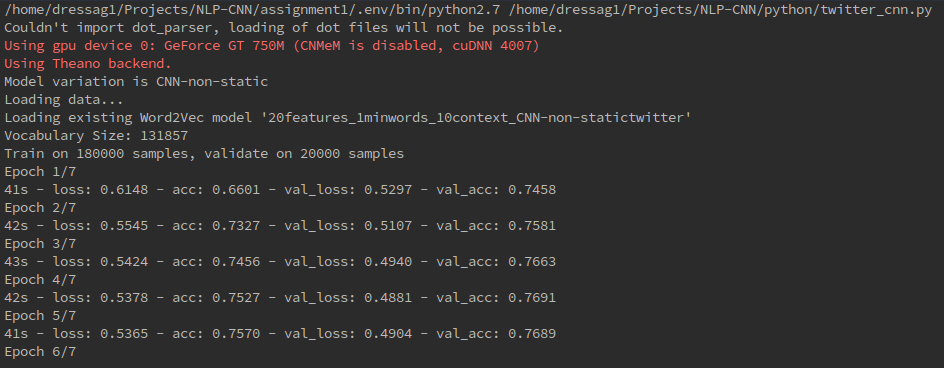
\includegraphics[scale=.4]{training.png}
	\caption{Output from Keras when training a \ac{cnn}.}
	\label{fig:training}
\end{figure}

\section {Datasets of Interest}

In the following sub-sections I cover two datasets that I investigated for sentiment analysis throughout the semester. The first is a IMDB Movie Reviews and the second is the Twitter Sentiment140 dataset. In both cases I compare the performance of \ac{cnn}'s trained on Word2Vec embeddings against Random Forest Classifier Trained on \ac{bow} embeddings.

\subsection{IMDB Movie Review Dataset}

IMDB is online database that contains information about movies, television shows, casts, summaries, and movie reviews. The IMDB dataset is a collection of movie reviews by both professional critics and normal individuals. Movie reviews are a great source for sentiment analysis in \ac{nlp} as getting labeled data is generally easier. Fans and critics upload reviews and  label the review through the use of a star or number system.

\subsubsection {Dataset Description}

The dataset came with training and testing sets already defined. The training set contains 24722 labeled movie reviews while the test set contains 24723 reviews. Unfortunately the test set is unlabeled. This dataset was attained through a Kaggle Data Science Competition \cite{kaggle}. The competition has since ended, but the dataset is still available to download. Kaggle only provided labels for the training set as the dataset is used for a competition. For this reason, I had to split the training data to make my own training and test sets. The data was split 80\slash20 for training and testing respectively. This dataset contains a vocabulary size of 81322 words. The longest sequence length is 2633 words. The labels for the dataset are binary: positive or negative. 


%pos train: 9873
%neg train: 9905

%neg test = 2444
%pos test = 2500

\newpage
\subsubsection {Results and Discussion}
%train 18000, 2000 validation, 5000 test
%Vocabulary size = 81322 words

%accuracy:86.06 percent
%
%Confusion Matrices
%[[1897  581]
%[ 116 2406]]
%
%[[ 0.77  0.23]
%[ 0.05  0.95]]

In Tables \ref{table:c_imdb} and \ref{table:b_imdb} are the results for a \ac{cnn} trained on Word2Vec embeddings and a random forest classifier trained on \ac{bow}. The classifiers were trained for sentiment analysis. Negative means that the review of interest was not liked by writer. Positive means that the author of the review liked the movie a lot. Performance accuracy for both classifiers are relatively similar, but the \ac{cnn} approach is roughly 2\% more accurate. An interesting observation is that the \ac{cnn} approach has higher precision for classifying positive movie reviews. \ac{bow} is very uniform in its classification ability. It would be interesting to explore a movie review dataset that has finer sentiment labels such as a scale from 1-5 with 3 being neutral.


\begin{table}[!htbp]
	\centering
	\begin{tabular}{l|l|c|c|c}
		\multicolumn{2}{c}{}&\multicolumn{2}{c}{True Values}&\\
		\cline{3-4}
		\multicolumn{2}{c|}{}&Negative&Positive&\multicolumn{1}{c}{}\\
		\cline{2-4}
		\multirow{2}{*}{Predictions}& Negative & $0.77$ & $0.23$ & \\
		\cline{2-4}
		& Positive & $0.05$ & $0.95$ &\\
		\cline{2-4}
		%	\multicolumn{1}{c}{} & \multicolumn{1}{c}{Total} & \multicolumn{1}{c}{$a+c$} & \multicolumn{\
		%		1}{c}{$b+d$} & \multicolumn{1}{c}{$N$}\\
		
	\end{tabular}
	\caption{\ac{cnn} normalized confusion matrix for IMDB dataset. Total accuracy on the test dataset is 86.1\%.}
	\label{table:c_imdb}
\end{table}


%BOW results
%[[2101  397]
%[ 389 2113]]
%
%.84 .15
%.1554 .844
%
%accuracy 84.28 percent

\begin{table}[!htbp]
	\centering
	\begin{tabular}{l|l|c|c|c}
		\multicolumn{2}{c}{}&\multicolumn{2}{c}{True Values}&\\
		\cline{3-4}
		\multicolumn{2}{c|}{}&Negative&Positive&\multicolumn{1}{c}{}\\
		\cline{2-4}
		\multirow{2}{*}{Predictions}& Negative & $0.84$ & $0.16$ & \\
		\cline{2-4}
		& Positive & $0.16$ & $0.84$ &\\
		\cline{2-4}
		%	\multicolumn{1}{c}{} & \multicolumn{1}{c}{Total} & \multicolumn{1}{c}{$a+c$} & \multicolumn{\
		%		1}{c}{$b+d$} & \multicolumn{1}{c}{$N$}\\
		
	\end{tabular}
	\caption{\ac{bow} normalized confusion matrix for IMDB dataset. Total accuracy on the test dataset is 84.3\%.}
	\label{table:b_imdb}
\end{table}



\subsection{Twitter Sentiment Dataset}

Twitter is a social networking website \cite{twitter} where users can post 140 character messages on their accounts. Once the message is posted it is completely open to the entire Twitter user base. Twitter has evolved as a means of rapidly sharing information. For example, a company may choose to post that a new product is available on Twitter in addition to their website to reach a larger user base. Twitter posts are rich with sentiment and make it a good source for sentiment analysis.

\subsubsection {Dataset Description}

To date there are no large hand labeled twitter datasets available for sentiment analysis. This led several Stanford Researchers \cite{Go_Bhayani_Huang_2009} to collect and build their own dataset called Sentiment140 \cite{sentiment140}. Labeling individual tweets for sentiment is a very tedious task, so the authors came up with a very creative way to mine positive and negative tweets. Twitter data was collected through the Twitter \ac{api} and labeled by using positive and negative emoticons. For example, if a tweet included a smiley face ``:)" it was considered positive. If a tweet contained both a positive and negative emoticons the tweet was not used. The dataset was collected between April 6, 2009 to June 25, 2009.

In total there are 1.6 million tweets used for training. The number of positive and negative tweets are equal for training. The test data is much smaller containing only 500 tweets. Interestingly neutral tweets are also provided, but no neutral tweets were provided in the training set. For this reason, the neutral tweets were not used. This brought the test set down to 359 tweets. The tweets used for testing were hand labeled, where as the training tweets were mined. This dataset contains a vocabulary size of 564692 words. The longest sequence length is 52 words. 

%Used same CNN network structure \cite{kim2014convolutional}

\subsubsection {Results and Discussion}

In Tables \ref{table:c_twitter} and \ref{table:b_twitter} are the results for \ac{cnn} trained on Word2Vec embeddings and a random forest classifier trained on \ac{bow}. As with the IMDB dataset the \ac{cnn} outperforms the \ac{bow} approach by about 3\% accuracy. In both cases here the classifiers have a harder time classifying the positive tweets (calling positive tweets negative).


\begin{table}[!htbp]
	\centering
	\begin{tabular}{l|l|c|c|c}
		\multicolumn{2}{c}{}&\multicolumn{2}{c}{True Values}&\\
		\cline{3-4}
		\multicolumn{2}{c|}{}&Negative&Positive&\multicolumn{1}{c}{}\\
		\cline{2-4}
		\multirow{2}{*}{Predictions}& Negative & $0.80$ & $0.20$ & \\
		\cline{2-4}
		& Positive & $0.23$ & $0.77$ &\\
		\cline{2-4}
		%	\multicolumn{1}{c}{} & \multicolumn{1}{c}{Total} & \multicolumn{1}{c}{$a+c$} & \multicolumn{\
		%		1}{c}{$b+d$} & \multicolumn{1}{c}{$N$}\\
		
	\end{tabular}
	\caption{\ac{cnn} normalized confusion matrix for Sentiment140 dataset. Total accuracy on the test dataset is 78.6 \%.}
	\label{table:c_twitter}
\end{table}

\begin{table}[!htbp]
	\centering
\begin{tabular}{l|l|c|c|c}
	\multicolumn{2}{c}{}&\multicolumn{2}{c}{True Values}&\\
	\cline{3-4}
	\multicolumn{2}{c|}{}&Negative&Positive&\multicolumn{1}{c}{}\\
	\cline{2-4}
	\multirow{2}{*}{Predictions}& Negative & $0.78$ & $0.22$ & \\
	\cline{2-4}
	& Positive & $0.27$ & $0.73$ &\\
	\cline{2-4}
%	\multicolumn{1}{c}{} & \multicolumn{1}{c}{Total} & \multicolumn{1}{c}{$a+c$} & \multicolumn{\
%		1}{c}{$b+d$} & \multicolumn{1}{c}{$N$}\\

\end{tabular}
	\caption{\ac{bow} normalized confusion matrix for Sentiment140 dataset. Total accuracy on the test dataset is 75.4\%.}
	\label{table:b_twitter}
\end{table}

%Bow
%[[147  41]
%[ 47 124]]
%[[ 0.78  0.218]
%[ 0.27  0.73]]

%Total of 75.4\% accuracy.


%after 7 epochs
%rand - 78 %
%cnn-non-static - 75 % 75.98 %
%cnn- static

%cnn-non-static on 359 test exemplars after 7 epochs
%[[130  47]
%[ 37 145]]
%
%[[ 0.73  0.27]
%[ 0.2   0.8 ]]

%100 features
%[[142  35]
%[ 42 140]]
%[[ 0.8   0.2 ]
%[ 0.23  0.77]]


\section {Conclusion}
\ac{cnn}s are a very power classification tool for learning useful features for both images and sentiment analysis. In both datasets that were tested \ac{cnn}s outperformed the standard \ac{bow} approach. While \ac{cnn}s perform better the do not offer the same level of performance gains achieved in object detection and recognition. In the case of object recognition \ac{cnn}s have a biological inspired source where as text understanding in the human mind likely does not use a form of convolution. In future work I would like to explore the use of \ac{rnn}s for sentiment analysis as newer research indicates that they offer better performance. 

\newpage
\appendix
\section{\\Project Development Schedule} \label{App:AppendixA}
% the \\ insures the section title is centered below the phrase: AppendixA
\begin{figure}[htbp!]
	\centering
	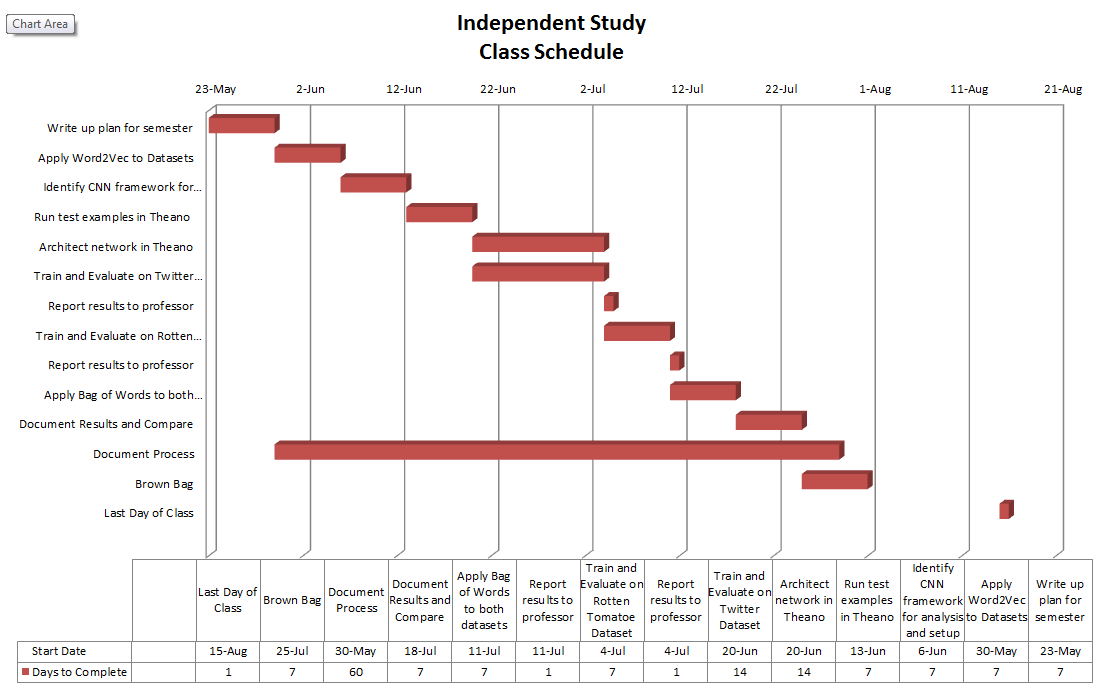
\includegraphics[scale=.5]{gantt.PNG}
	\caption{Project Development Schedule}
%	\label{fig:schedule}
\end{figure}

\newpage
\section{\\Word2Vec Feature Plot} \label{App:AppendixB}
% the \\ insures the section title is centered below the phrase: Appendix B

\begin{figure}[htbp!]\centering
	\centering
	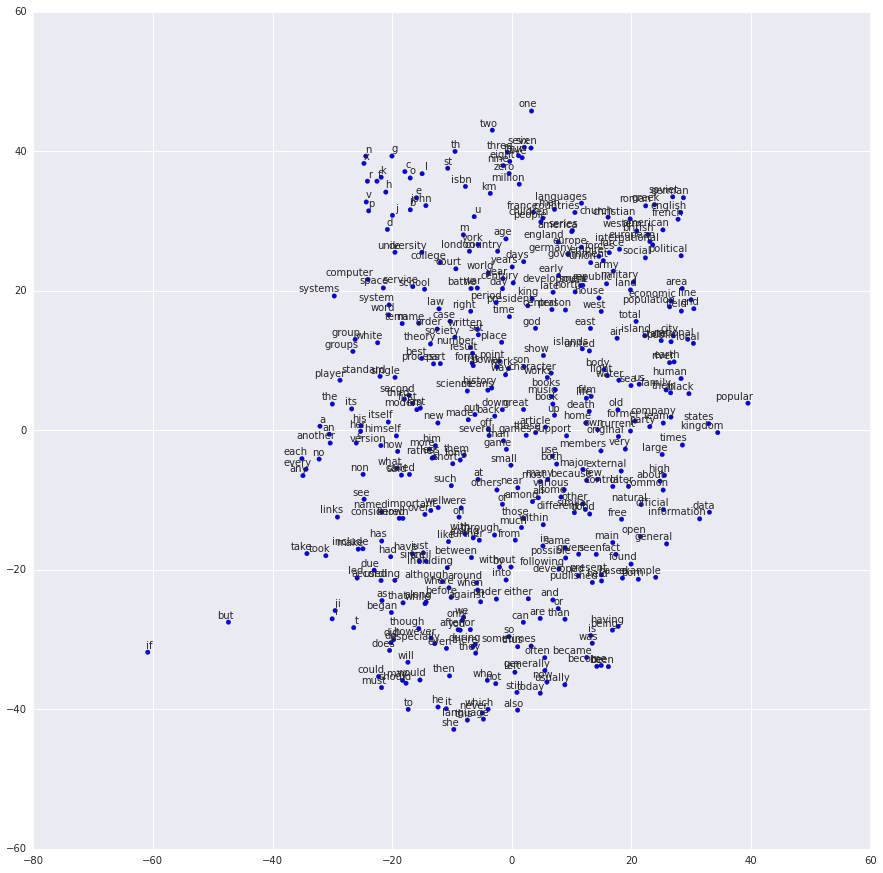
\includegraphics[scale=.5]{tsne.png}
	\caption{Word2Vec vector plot showing that similar words appear near each other in the feature space \cite{tensorflow}.}
	%	\label{fig:schedule}
\end{figure}

\newpage
\bibliography{Austin_Dress_NLP_CNN_Summer_2016.bib}
\bibliographystyle{plain}

\end{document}
